\section{Sieve of Eratosthenes}

The sieve of Eratosthenes is an ancient algorithm for findilg all primes up to a
upper limit called Max. This algorithm is very old and was first described to 
Eratosthenes of Cyrene, who lived in the 3rd century BC. 
\cite{eratosthenes} 
This is done by iteratievely calculate multiples of a 
iterator $k$ and marking these multiples. This iterator is is $2$ in the beginning
and when all multiples of $2$ is marked, find the first unmarked number i.e $3$
and repeat until $k^2 >$ Max.

This implementation attempted to stay as true to the original algorithm as 
possible and thus first computes the primes from 2 to $\sqrt{max}$ in a serial 
fashion. Once complete these 'seed' primes are stored in an array.
The remaining numbers (that being from $\sqrt{\text{max}}$ to max) are then 
split amongst the number of threads. This is done by dividing the amount of 
remaining numbers by the number of threads and flooring the result. If the 
aforementioned remaining list is divisible by numberOfThreads without remainder, 
work is distributed equally (and therefore fully \textit{balanced}). If however the 
result is not fully divisible, the final thread picks up the extra cycles 
(thus leaving it in an almost equal split for all but one of the threads) and 
completes the calculation. 

\begin{figure}
    \centering
    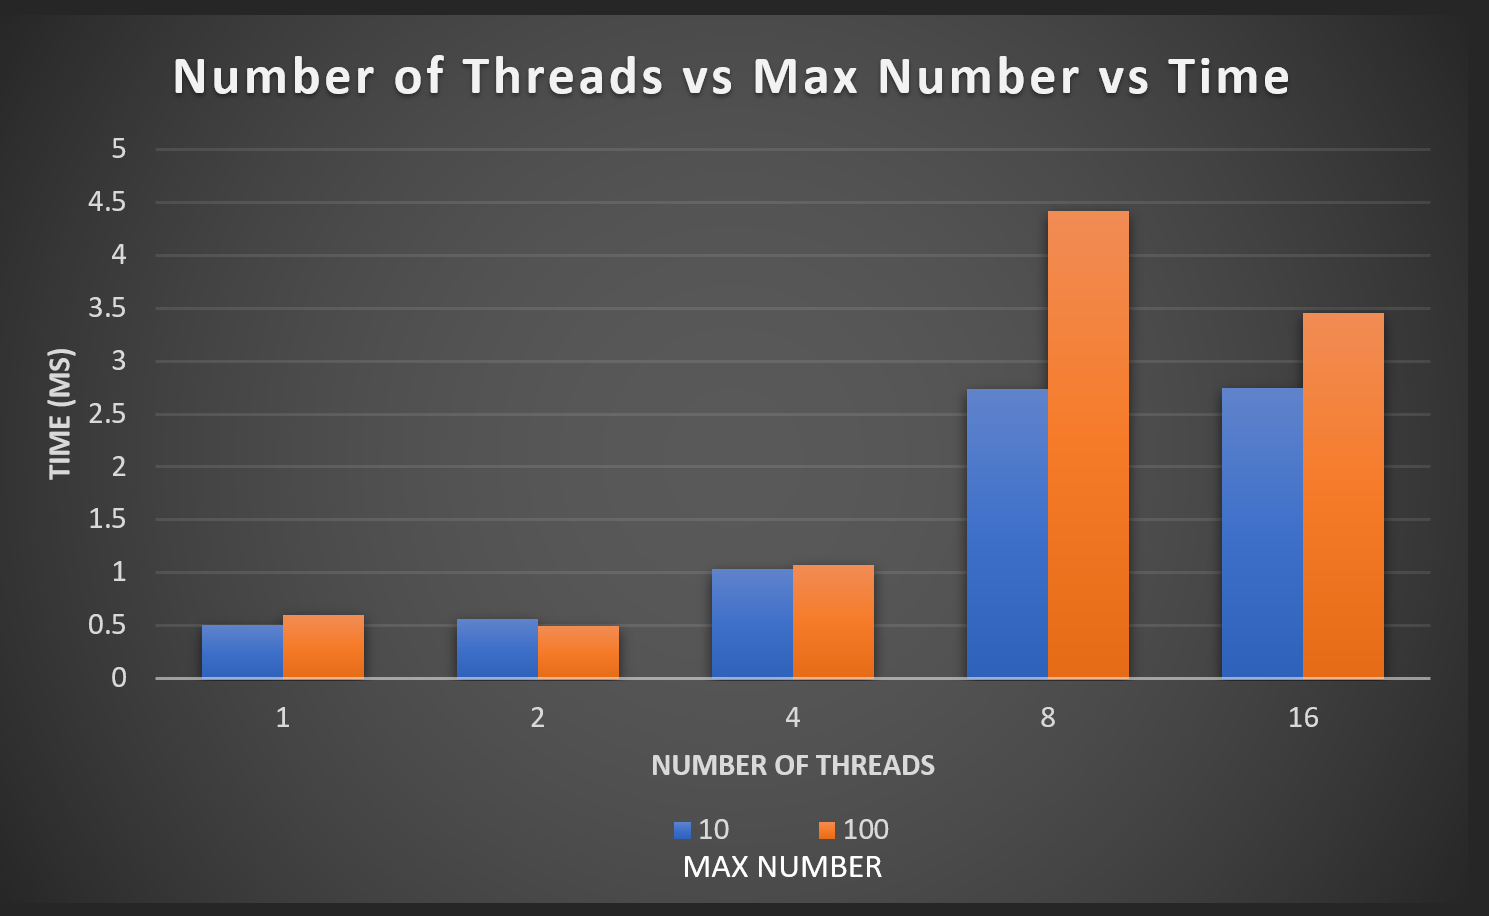
\includegraphics[width=\linewidth]{Figures/maxNumLow.png}
    \caption{Max $\in \{10, 100\}$ and $T \in \{1, 2, 4, 8, 16\}$}
    \label{fig:maxnumlow}
\end{figure}

Mathematically given the fact the partition size is 
constant (for almost all cases) and the seed values are constant, the work for 
each thread is almost equal (as the checks would equate to 
\textit{for each number in range, check if number is divisible by any number in seeds}). Therefore the 
max-checks for each thread is \textit{rangeLength * numberOfSeeds}. A potential 
inequality argument may be made that the actual checks done may be slightly 
quicker in one thread vs another (as one thread may hold a range with many 
numbers divisible by 2, which would result in far quicker tests). This argument 
is valid, however testing has not shown this to be impactful in any meaningful 
way.

Furthermore no synchronization between threads were utilized in this solution. 
The simple reasoning behind this is that no thread operates on the same block 
of memory that another thread operates on. As the results array is a contiguous 
block of memory, with each element getting a distinct memory address, it 
therefore follows that each element can be interacted with independently of each 
other. Since the algorithm partitions the remaining numbers into distinct chunks 
with no overlap, no thread contains or interacts with numbers out of its chunk, 
which therefore follows that no thread interacts with elements being touched by 
another thread (in terms of the 'result' array.) One \textit{could} add a mutex lock 
on writes to results, however the overhead of the lock checks would provide no 
real benefit as the algorithm ensures that each block works independently. 

\begin{figure}
    \centering
    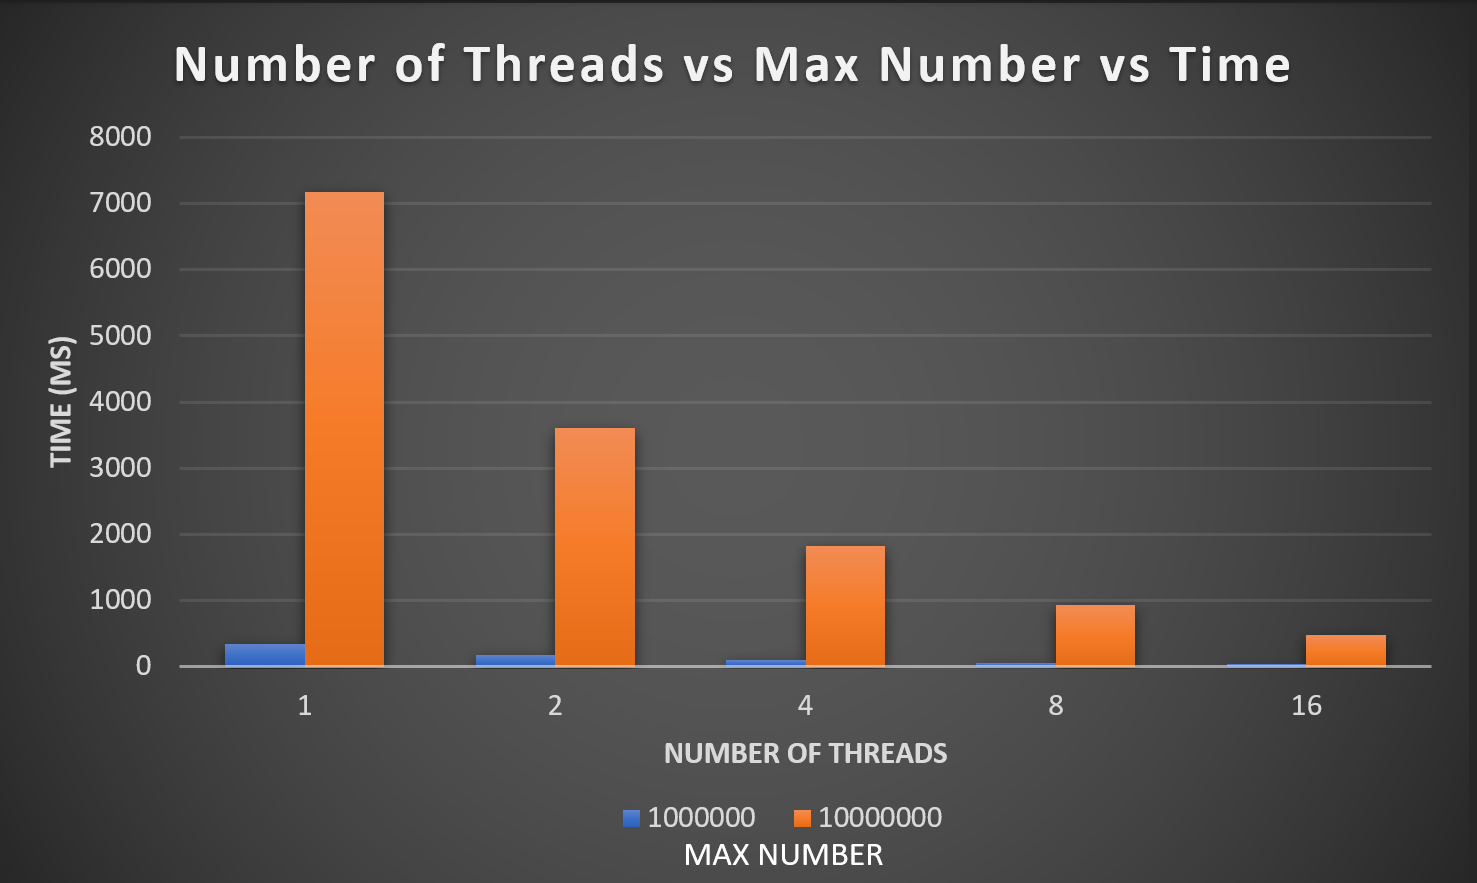
\includegraphics[width=\linewidth]{Figures/maxNumHigh.png}
    \caption{Max $\in \{10^6, 100^7\}$ and $T \in \{1, 2, 4, 8, 16\}$}
    \label{fig:maxnumhigh}
\end{figure}

The only piece of common-shared memory between the threads is the 'seeds' array. 
This common interaction is only done in a \textbf{read-only} fashion. And since the 
seeds array is computed once in a serial fashion \textit{before} the threads spin-up, 
we know that its value is written once and never altered after. Therefore there 
is no issue with multiple threads reading its value at the same time. 
For safety's sake we could add a read-write lock at this point, however the 
overhead of the lock will slow down the program for a case that is impossible 
given the design of the algorithm. As mentioned above, there is no real communication between sub-threads of the 
main thread (as they operate independently), with the only real communication 
occuring between the main thread and individual sub-threads, where sub-threads 
would update distinct shared-memory locations and for the main-thread to wait 
for sub-threads to complete and join to the main thread.

\subsection{Results}

\begin{figure}
    \centering
    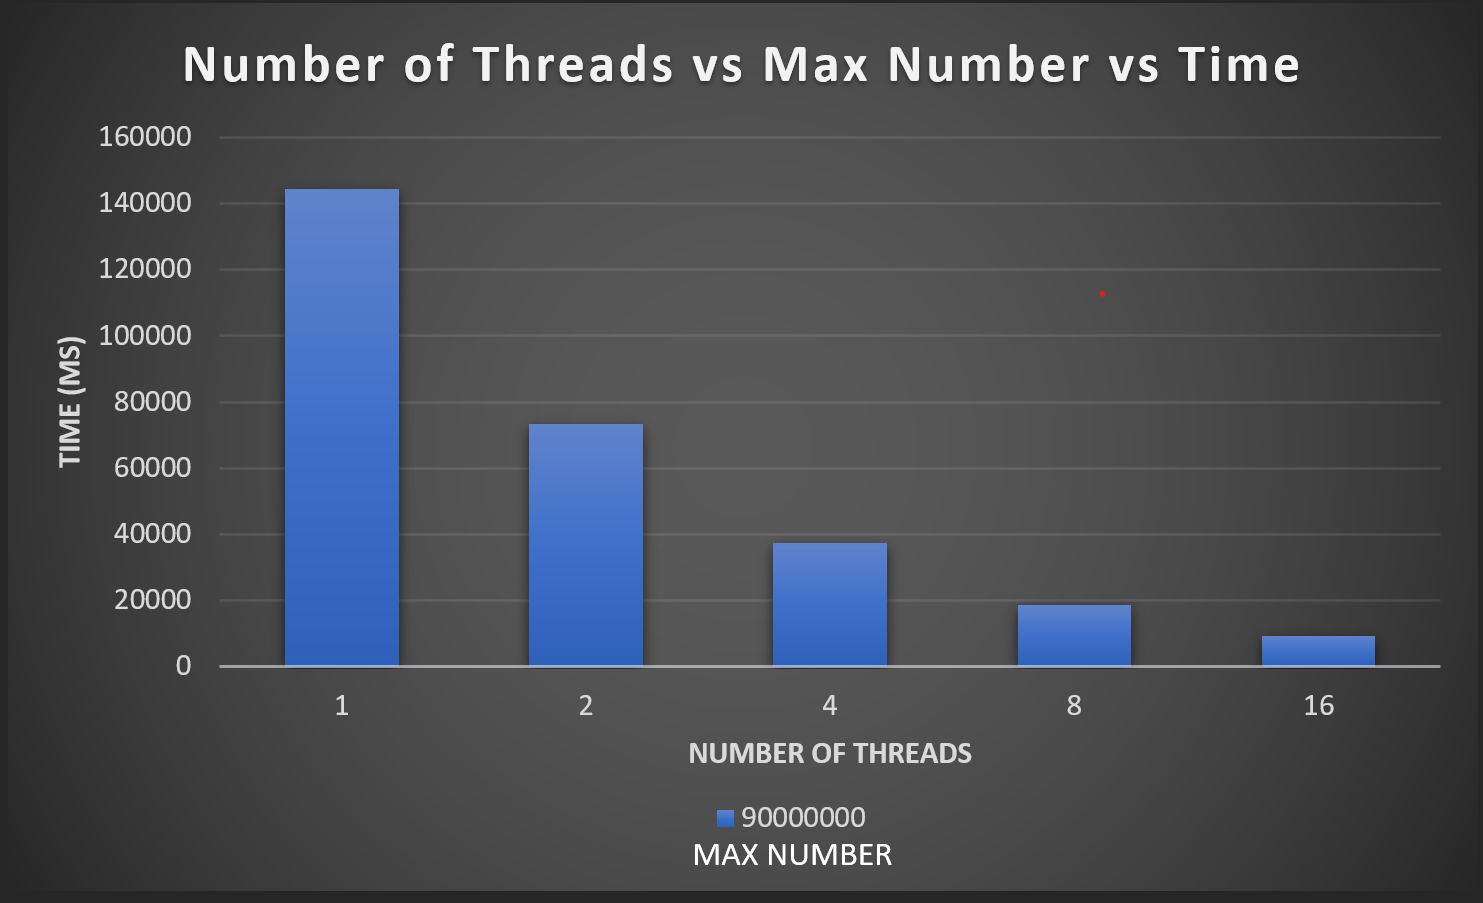
\includegraphics[width=\linewidth]{Figures/maxNumVHigh.png}
    \caption{Max $\in \{10, 100\}$ and $T \in \{1, 2, 4, 8, 16\}$}
    \label{fig:maxnumvhigh}
\end{figure}

As seen in the figure \ref{fig:maxnumlow}, at lower maxNums 
(that being $10$ or $100$), we see that the 
time actually increase as we add more threads. This seems to be due to the 
system overhead of managing threads (creation, tracking and freeing) and the 
design of the algorithm (which for smaller numbers creates many more partitions
that is actually required, thus threads are barely doing any work). However as 
we increase maxNum into the millions (in our testing $10^6$ and $10^7$) as seen 
in figure \ref{fig:maxnumhigh}, 
we see that the time taken to compute the primes scales linearly as we increase 
the amount of threads (that is 2 threads takes about 50\% of the time that 1 
thread takes, with 4 threads taking 25\% of the time).This result is further 
demonstrated when looking at the computational results when maxNumber is 
$9\times10^7$ as seen in figure \ref{fig:maxnumvhigh}. In conclusion, this exercise demonstrates the impact that an algorithm 
and chosen parameters ultimately decides when parallelism can make a difference 
(and by how much) to your application.



